In this section we study the structure of pairs of pants.

An oriented closed surface homeomorphic to $$\{(x,y)|x^2+y^2\leq 4\}-\{(x,y)|(x-1)^2+y^2< \frac{1}{4}\}\cup\{(x,y)|(x+1)^2+y^2< \frac{1}{4}\}$$  is called  a pair of pants. 

\begin{figure}[h]
    \centering
    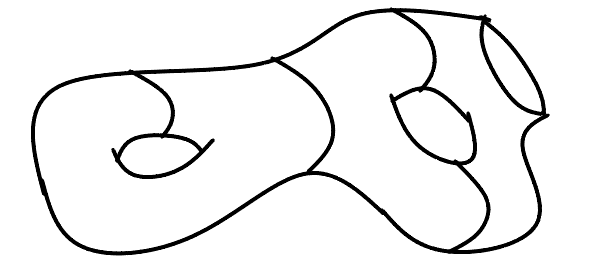
\includegraphics[width=3 in]{picture/pantsde.png}
    \caption{Case of $g=2,n=1$}
    \label{fig:pantsde}
\end{figure}

For a Riemann surface $S_{g,n}$ of genus $g$ with $n$ geodesic boundary components, take disjoint, non-peripheral simple closed geodesics $\Gamma=\{\gamma_1,\gamma_2,\cdots,\gamma_r\}$ as much as possible and cut   $S_{g,n}$ along them. See Figure \ref{fig:pantsde}. The only Riemann surface of negative  curvature admitting  no non-peripheral simple closed geodesic is just $S_{0,3}$ or a pair of pants. Notice that $\chi(S_{0,3})=-1$, $\chi(S_{g,n})=2-2g-n$, so $\Gamma$ contains $3g+n-3$ geodesics and $S_{g,n}$ will be cut into $2g-2+n$ pairs of pants.


It has been mentioned that for a closed oriented surface with boundary negative curvature, each homotopy class of curves contains a unique geodesic. Similarly, consider the shortest curves with ends on two of the boundaries, the three geodesics cut the pants into  geodesic hexagons with six right angles. 

The complex structure of a  pair of pants and the lengths of three boundary components decide each other by the following lemma. \cite{Imayoshi1992An}

\begin{lemma}\label{uni}
 Given $l_i>0,i=1,2,3$, there is a unique right angled geodesic hexagon with six sides $a_1,b_1,a_2,b_2,a_3,b_3$ satisfying $l(b_i)=l_i$.
 \end{lemma}
 
 \begin{proof}
Firstly, take five geodesics $a_1,b_1,a_2,b_2,a_3$ in order, and adjacent geodesics meet at right angles.
Set the distance between $a_1$ and $a_2$ or the length of arc on $b_1$ cut by $a_1$ and $a_2$ to be $l_1$, and the distance between $a_2$ and $a_3$ to be $l_2$. Now consider the distance $l$ between $b_1$ and  $b_2$.
If $l$ approaches $\infty$, then the distance between $a_1$ and $a_3$ goes $\infty$, and goes $0$ as $l$ approaches $0$.
Therefore appropriate $l$ will satisfy that the distance between $a_1$ and $a_3$ is $l_3$.
Then  the existence of the hexagon is shown. 


\begin{figure}[h]
    \centering
    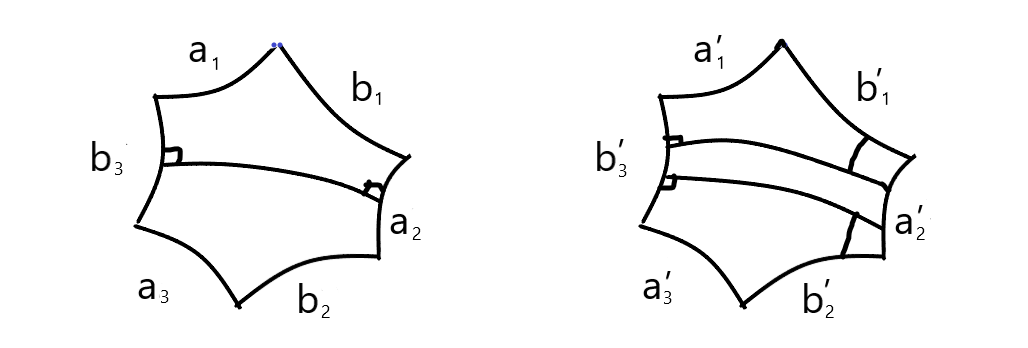
\includegraphics[width=4in]{picture/uniqueness.png}
    \caption{Uniqueness}
    \label{fig:uniqueness}
\end{figure}

For uniqueness, notice that if two right angled geodesic hexagons have same edge lengths, then by passing to $\operatorname{PSL}(2,R)$ they are coincident. Consider two right angled geodesic hexagons $H$ and $H^\prime$ with edges $a_1,b_1,a_2,b_2,a_3,b_3$ and $a_1^\prime,b_1^\prime,a_2^\prime,b_2^\prime,a_3^\prime,b_3^\prime$. Assume that $l(a_i)=l(a_i^\prime)$, and $l(b_3)<l(b_3^\prime)$. There  exists unique point pair $(p,q)$ on $a_2$ and $d_3$ such that $d(p,q)=d(a_2,b_3)$. The geodesic from  $p$ to $q$ lies entirely inside $H$, since otherwise there is a triangle with two right angles, which is impossible by the Gauss-Bonnet theorem.  If the distance from $q$ to $a_1$ and $a_3$ is $s$ and $s^\prime$, then consider the points $q_1$ and $q_2$ of distance $s$ and $s^\prime$ from $a_1^\prime$ and $a_3^\prime$ separately. See Figure \ref{fig:uniqueness}. Denote the geodesics passing $b_3^\prime$ at $q_1$ and $q_2$ orthogonally  by $l_1,l_2$, then $l_1\cap l_2\cap H^\prime=\emptyset$ by the same argument. $l_1$ and $l_2$ intersect with $a_2^\prime$ at $e_1$ and $e_2$. Then $l(a_2)=d(b_1,b_2)= d(b_1,q)+d(q,b_2)\leq d(e_1,b_1^\prime)+d(e_2,b_2^\prime)<d(b_1^\prime,b_2^\prime)=l(a_2^\prime)$, which is contradictory. 
\end{proof} 
 
 
 From the above lemma, each pair of pants admits a reflection $\sigma$ of order two, which exchanges the corresponding points of two hexagons.  
 
\begin{figure}[h]
    \centering
    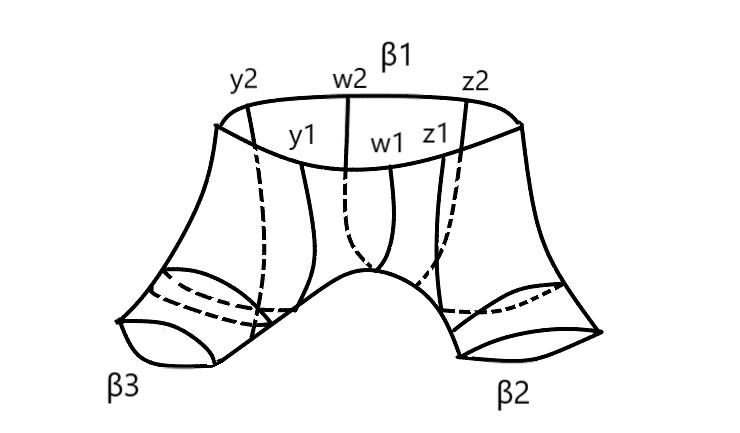
\includegraphics[width=3 in]{picture/pantshy.png}
    \caption{Special geodesics orthogonal to $\beta_1$}
    \label{fig:pantshy}
\end{figure}
 
 Denote the three boundary components by $\beta_i,i=1,2,3$. Now consider the geodesics with ends on $\beta_1$. there are two geodesics  meeting $\beta_1$ orthogonally and spiraling around  $\beta_3$. Set the intersecting points with $\beta_1$ to be $y_1,y_2$. Similarly, set $z_1,z_2$ to be the intersecting points of $\beta_1$ and geodesics spiraling around $\beta_2$. Besides, there is a unique geodesic with two end points on $\beta_1$ and perpendicular to $\beta_1$. Denote the two end points by $w_1,w_2$. The six points may be arranged by $y_1,w_1,z_1,z_2,w_2,y_2$ in succession as in Figure \ref{fig:pantshy}.
 
 By the symmetry of the pair of pants, $\sigma(y_1)=y_2,\sigma(w_1)=w_2,\sigma(z_1)=z_2$.
 

 \begin{figure}[h]
     \centering
     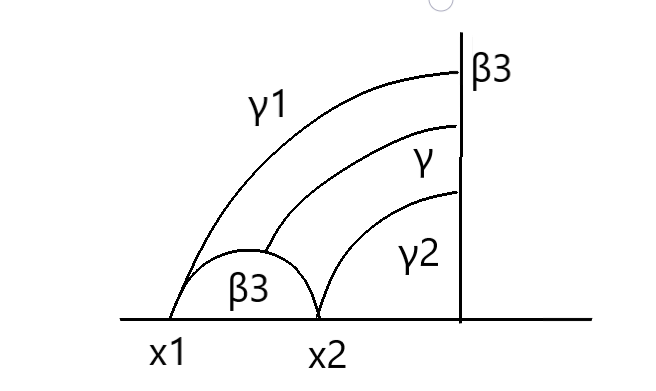
\includegraphics[width=3 in ]{picture/touying.png}
     \caption{Projection of $\beta_3$ to $\beta_1$}
     \label{fig:touying}
 \end{figure}
 
 
 \begin{remark}
 Lift $\beta_1$ to $x=0$ on the universal covering. Consider the one lifting $\gamma$ of the shortest geodesic connecting $\beta_1$ and $\beta_3$.Among all the lifting of $\beta_3$, denote the one meeting $\gamma$ first by $\alpha$. Project the two end points $x_1,x_2$ on $x$-axis to $x=0$ along $\gamma_1,\gamma_2$, and the projections of $\gamma_1,\gamma_2$ are the geodesics meeting $\beta_1$ orthogonally and spiraling around $\beta_3$.
 \end{remark}
 
 Use $x_1,x_2,x_3$ to denote the lengths of $\beta_1,\beta_2,\beta_3$ and $C(x_1,x_2,x_3)$ to denote the corresponding pair of pants. Define $R(x_1,x_2,x_3)$ to be the length of the curve $\overline{y_1y_2}$ containing $w_1,w_2,z_1,z_2$, and define  $D(x_1,x_2,x_3)$ to be the sum of  length of the curves $\overline{y_1w_1z_1}$ and $\overline{y_2w_2z_2}$.   The length of  $\overline{y_1w_1z_1}$ and $\overline{y_2w_2z_2}$ are equal by the symmetry action of $\sigma$.
 
 \begin{remark}
 By the reflection $\sigma$ of $C(x_1,x_2,x_3)$, 
 $$D(x_1,x_2,x_3)=D(x_1,x_3,x_2),$$ and $$
 D(x_1,x_2,x_3)=R(x_1,x_2,x_3)+R(x_1,x_3,x_2)-x_1.$$ Meanwhile,
 $$x_1-R(x_1,x_2,x_3)$$ is equal to the length of the projection of $\beta_3$.
 \end{remark}
 
 \begin{lemma}\label{DR}
  \begin{equation}\label{DD}
  D(x,y,z)=2\log \left(\frac{e^{\frac{x}{2}}+e^{\frac{y+z}{2}}}{e^{\frac{-x}{2}}+e^{\frac{y+z}{2}}}\right)
  \end{equation}
 \begin{equation}\label{R}
     R(x,y,z)=x-\log \left(\frac{\cosh(\frac{y}{2})+\cosh (\frac{x+z}{2})}{\cosh(\frac{y}{2})+\cosh (\frac{x-z}{2})}\right)
 \end{equation}
 \end{lemma}
 
 \begin{lemma}\label{tri}
  For a geodesic trirectangle with edges of length $a,b,\alpha,\beta$ in order, and the angle between $\alpha$ and $\beta$ is $\phi$, with the rest three right angles, there is an identity:
  \begin{equation}\label{rect}
      \cos\phi=\sinh a\cdot \sinh b=\tanh\alpha\cdot \tanh\beta.
  \end{equation}
 \end{lemma}
 
 \begin{lemma}\label{hex}
   For a right angled geodesic hexagon with edges of length $a,\beta,c,\alpha,b,\gamma$,   there is an identity:
   \begin{equation}
       \cosh c=\sinh a\cdot\sinh b\cdot\cosh \gamma-\cosh a\cdot\cosh b.
   \end{equation}
 \end{lemma}
 
 \begin{remark}
 Such trigonometry formulas can be referred in the Formula Glossary part  in \cite{Buser}. They are all obtained by comparing the composition  of different isometries on hyperboloid $\{(x,y,z)\in \mathbb{R}^3|x^2+y^2-z^2=-1\}$.  
 \end{remark}
 
 \begin{proof}[Proof of lemma \ref{DR}]
 Consider the picture in Figure \ref{fig:touying}, apply the equation \ref{rect} to the trirectangle bounded by $\beta_3,\gamma_1,\gamma,\beta_1$, and $\beta_3,\gamma_2,\gamma,\beta_1$, then $$R(x,y,z)=x-d(\gamma,\gamma_1)-d(\gamma,\gamma_2)=x-2\sinh^{-1} \left(\frac{1}{\sinh(d(\beta_1,\beta_3))}\right).$$
 
 Cut the pair of pants into two right angled hexagons and apply the lemma \ref{hex}. Notice that the lengths of six edges are $d(\beta_1,\beta_3)$,$\frac{z}{2}$, $d(\beta_3,\beta_2)$, $\frac{y}{2}$, $d(\beta_2,\beta_1)$, $\frac{x}{2}.$ So $d(\beta_1,\beta_3)$ only depends on the lengths of three boundary components by 
 $$ 
 \cosh(\frac{y}{2})=\sinh(\frac{x}{2})\sinh(\frac{z}{2})\cosh(d(\beta_1,\beta_3))-\cosh(\frac{x}{2})\cosh(\frac{z}{2}).
 $$
 
 Since $$\sinh^{-1} x=\log \left(x+\sqrt{x^2+1}\right),$$ the equation (\ref{DD}) follows by  $$
 \begin{aligned}
 x-R(x,y,z)=&2\log\left(\frac{1}{\sinh(d(\beta_1,\beta_3))}+\sqrt{1+\frac{1}{\sinh^2(d(\beta_1,\beta_3))}}\right)\\
 =&\log\left(\frac{(1+\cosh(d(\beta_1,\beta_3)))^2}{\sinh^2(d(\beta_1,\beta_3))}\right)\\
 =&\log\left(\frac{\cosh(d(\beta_1,\beta_3))+1}{\cosh(d(\beta_1,\beta_3))-1}\right)\\
 =&\log\left(    \frac{
 \cosh(\frac{y}{2}) +\cosh(\frac{x}{2})\cosh(\frac{z}{2}) +\sinh(\frac{x}{2})\sinh(\frac{z}{2})     }
 {   \cosh(\frac{y}{2}) +\cosh(\frac{x}{2})\cosh(\frac{z}{2}) -\sinh(\frac{x}{2})\sinh(\frac{z}{2})   }  \right)\\
 =&\log\left(\frac{   \cosh(\frac{y}{2})+\cosh(\frac{x+z}{2})   }{  \cosh(\frac{y}{2}) +\cosh(\frac{x-z}{2})    }\right).\\
 \end{aligned}
 $$
Then (\ref{DD}) follows by $D(x,y,z)=R(x,y,z)+R(x,z,y)-x$.
 \end{proof}
 
 In section \ref{wpvolume} the differentials of $D$ and $R$ will be integrated. Some of calculations are presented here.
 
 \begin{lemma}\label{DRpp}
   Define $$H(x,y)=\frac{1}{1+e^{\frac{x+y}{2}}}+\frac{1}{1+e^{\frac{x-y}{2}}},$$ then the derivatives of $D$ and $R$  with respect to $x$ are  given by:
   \begin{equation}\label{pp1}
       \frac{\partial}{\partial x}D(x,y,z)=H(y+z,x),
   \end{equation}
    and 
    \begin{equation}\label{pp2}
        \frac{\partial }{\partial x }R(x,y,z)=\frac{1}{2}(H(z,x+y)+H(z,x-y)).
    \end{equation}
    
 \end{lemma}
 
 \begin{proof}
 By direct calculation $$\frac{\partial}{\partial x}D(x,y,z)=\frac{e^{\frac{x}{2}}}{e^{\frac{x}{2}}+e^{\frac{y+z}{2}}}+ \frac{e^{-\frac{x}{2}}}{e^{-\frac{x}{2}}+e^{\frac{y+z}{2}}}=H(y+z,x).$$
 
  Although $D,R$ is defined on $\mathbb{R}_+^3$,   the relationship holds formally:
    \begin{equation}\label{RDD}
       R(x,y,z)=\frac{1}{2}( D(x,y,z)+D(x,-y,z)).
    \end{equation}.
    
    (\ref{pp2}) follows it and (\ref{pp1}).
    This relationship can be checked as follows:
    $$
    \begin{aligned}
    &D(x,y,z)+D(x,-y,z)\\
    =&2\log\left(\frac{\cosh(\frac{x-y-z}{4})}{\cosh(\frac{x+y+z}{4})}\right)+2\left(\frac{x+y+z}{4}-\frac{y+z-x}{4}\right)        \\
    +& 2\log\left(\frac{\cosh(\frac{x+y-z}{4})}{\cosh(\frac{x-y+z}{4})}\right) +2\left(\frac{x-y+z}{4}-\frac{-y+z-x}{4}\right)          \\
    =&2x-2\log\left(\frac{   \cosh(\frac{x+y+z}{4})\cosh(\frac{x+z-y}{4})          }{  \cosh(\frac{x+y-z}{4})\cosh(\frac{y+z-x}{4})            }\right)\\
    =&2R(x,y,z)\\
    \end{aligned}
    $$
    
 \end{proof}
 
 \begin{remark}
 Since the function $R$ and $D$ are closely related to the geometry of the corresponding pair of pants, it will help to understand them by explaining  the  asymptotic behavior of $D$ and $R$ as $x,y,z$ approach $0$ or $\infty$ in geometry.
 \end{remark}
 
